\section{Serverless Control Plane Research}
\label{sec:platform-enhance}

\mhead{Cold Start Mitigation}
The FaaS computing paradigm sees providers running user code on-demand when a request comes in, and importantly deciding \emph{where} it should run. 
Each invocation must be run in isolation from co-located invocations and must ensure provider control over system resources.
Both security goals are thus achieved by running each invocation in a sandboxed environment. 
Sandboxes are generally implemented using containers (such as Docker~\cite{docker-main}) or lightweight VMs (such as Firecracker~\cite{firecracker-nsdi20}) created on the server that runs the invocation.
Unfortunately, creation time for both any type of sandbox can be significant, adding latency to the in-flight request. 

Many techniques have been proposed to reduce the initialization overhead from such \emph{cold starts}.
Cold start invocations, because of the large initialization overheads, are typically $1-10\times$ larger than the function execution time.
%  which occurs when the function is run in an already initialized container which is cached in memory. 
% They can be mitigated by skipping initialization entirely, by saving in memory and reusing the execution environment for subsequent invocations of the same function. 
We can mitigate this by the saving execution environment in memory and reusing it for subsequent invocations of the same function, skipping initialization entirely. 
Keeping the function \quotes{warm} thus allows a provider to amortize the startup cost across future invocations.

\mhead{Workload Characterization}
Published traces from major providers give a glimpse into the scale of serverless computing.
Shahrad et al.~\cite{shahrad_serverless_2020} publicized the first dataset of the functions served by Azure Fucntions, with a detailed characterization breakdown.
As seen in Figure~\ref{fig:wild-invokes}, invocation rates are \emph{extremely} heavy tailed.
% 0.1\% of functions account for half of all invocations, and the top 19\% account for a total of 99.6\% of invocations.
The most frequently invoked functions are executed several times a second, while the rarest perhaps once per day.
Because of this, a small portion, 19\% of functions, account for 99.6\% of invocations in Azure.
A paper describing an internal FaaS platform at Meta~\cite{sahraei2023xfaas}, showcased handling trillions of invocations daily and a similar skewed workload.

Several examples of functions are shown in Table~\ref*{tab:workloads}, these are taken from~\cite{functionbench}.
Functions have high variation in warm and cold-start times, with cold-start times being significantly higher.
Memory usage can range from a few dozen megabytes, to half a gigabyte, matching real-world data from~\cite{shahrad_serverless_2020}.
Control planes must be able to handle these high variations in frequency and resource usage, and treat all functions fairly.

\begin{figure}
  \begin{center}
    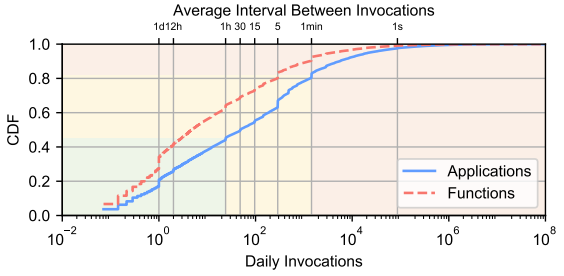
\includegraphics[width=.9\columnwidth]{./figures/wild-invocations.png}
    \caption{A CDF of daily invocations for functions. 
              Invocation frequencies range from sub-second to less than one per day. 
              Figure from~\cite{shahrad_serverless_2020}}
  \label{fig:wild-invokes}
\end{center}
\end{figure}

Functions exist in a data-driven architecture, being required to download inputs to handle each invocation.
The same group at Azure released another dataset in~\cite{romero2021faa}, focusing on data usage of functions and DAG applications.
They found a split of functions with some having high cloud storage usage and others almost none.
Surveys have shown that increasingly diverse applications are deployed on FaaS, which will rely on data movement by the platform~\cite{raza2021sok,hossein2022survey,eismann2020serverless}.
Some examples of these applications are explored in Section~\ref{sec:serverless-apps}.
% Control planes must cater to a host of diverse applications with equally varied runtime needs.

% The warm and cold time for different functions from the FunctionBench~\cite{kim_functionbench_2019} workload suite are shown in Table~\ref{tab:func-times}.
% The table shows the total execution latency when these functions are run on OpenWhisk.

\begin{table}
  \centering
  \caption{FaaS workloads are highly diverse in their resource requirements and execution times. The initialization time can be significant and is the cause of the cold-start overheads, and depends on the size of code and data dependencies.}
  \begin{tabular}{lrrr}
    \hline 
    Application & Mem size & Warm time (sec) & Cold-start time (sec) \\
    \hline
    % Web-serving & 64 MB & 2.4 s & 2 s \\
    % ML Inference (CNN) & 512 MB & 6.5 s & 4.5 s \\
    % Disk-bench (\texttt{dd})  & 256 MB & 2.2 s & 1.8 s \\
    % Floating Point & 128 MB & 2 s & 1.7 s \\
    % Image Manipulation & 300 MB & 9 s & 6 s \\
    % Matrix Multiply & 256 MB & 2.5 s & 2.2 s \\
    % Video Encoding & 500 MB & 56 s & 3 s \\
    Web-serving & 64 MB & 0.179 & 1.153 \\  
    ML Inference (CNN) & 512 MB & 2.211 & 7.833 \\
    Disk-bench (dd) & 256 MB & 1.068 & 2.944 \\  
    Floating Point & 128 MB & 0.083 & 1.432 \\  
    Image Manipulation & 300 MB & 4.806 & 5.268 \\  
    Matrix Multiply & 256 MB & 0.117 & 1.067 \\  
    AES Encryption & 128 MB & 0.587 & 2.064 \\  
    Video Encoding & 500 MB & 10.28 & 11.51 \\  
    JSON Parsing & 256 MB & 0.414 & 1.962 \\
    \hline
  \end{tabular}
  \label{tab:workloads}
\end{table}


\begin{comment}
\begin{table}
  \begin{tabular}{ c c c }
\hline
  Application & Warm Time (s) & Cold Time (s) \\ 
\hline
  Web-serving & 0.179 & 1.153 \\  
  ML Inference (CNN) & 2.211 & 7.833 \\
  Disk-bench (dd) & 1.068 & 2.944 \\  
  % float & 0.083 & 1.432 \\  
  % gzip & 0.406 & 1.033 \\  
  % image & 4.806 & 5.268 \\  
  Matrix Multiply & 0.117 & 1.067 \\  
  Sklearn Regression & 53.57 & 54.45 \\  
  AES Encryption & 0.587 & 2.064 \\  
  Video Encoding & 10.28 & 11.51 \\  
  JSON Parsing & 0.414 & 1.962 \\
\hline
\end{tabular}
\caption{FunctionBench~\cite{kim_functionbench_2019} functions run times' are significantly longer on cold starts. Ideally we want all of our functions to run warm to lower user latency. Cold starts also increase system load by creating runtime overhead.}
\label{tab:func-times}
%\vspace*{-0.4cm}
\end{table}
\end{comment}

\mhead{Reusing Initialization}
Performing multiple container startups of a function will involve executing the same startup procedures repeatedly: language runtimes, the OS of a micro-VM, etc.
Utilizing past startups by checkpointing the container at a known position and booting from there has proved promising in reducing cold start times~\cite{du2020catalyzer,vhive-asplos21}.
Memoization approaches that leverage existing containers to duplicate their state have proven highly effective~\cite{du2020catalyzer,wei2022booting}.

\mhead{Alternate Isolation Mechanisms}
While a simple implementation would run functions inside Docker containers~\cite{docker-main}, so long as isolation guarantees are upheld, using alternate mechanisms with faster start times is effective.
Directly optimizing the isolation mechanism~\cite{firecracker-nsdi20} or common libraries and language runtimes used by FaaS worklaods~\cite{carreira2021warm} both give immediate performance boosts. 
Running functions inside the worker's language runtime can dramatically reduce initialization times~\cite{vhive-asplos21,shillaker2020faasm,jia2021nightcore,du2020catalyzer}.
Security may be relaxed between functions in a larger application~\cite{akkus_sand_2018, dukic2020photons} allowing for the reuse of sandboxes.
%

\mhead{FaaS Resource Management}
Worker resources are not infinite, especially memory for keeping function sandboxes available.
Packing functions together can improve memory utilization~\cite{akhtar_cose_2020}.
Developers often over-assign memory, causing under-utilization, the control plane is in the perfect place to minimize this waste~\cite{eismann2021sizeless, mvondo2021ofc}.
Concurrent invocations of the same function has been reused to share resources, as isolation may be relaxed~\cite{stojkovic2023mxfaas}.

The initialization overheads of serverless functions and their repeated invocations have spawned a great deal of research into optimizing their resource management.
Recent surveys~\cite{faas-survey-jan-2022, raza2021sok, eismann2020serverless, hassan2021survey, mampage2021holistic} provide an overview of the challenges and solutions in this very active research area. 

% Locality for FaaS resource management has been explored in the form of function keep-alive policies~\cite{shahrad_serverless_2020}. 
% Once a container for a function is created and the function finishes execution, the container can be kept alive instead of immediately terminating it. 
% Subsequent invocations of the function can then \emph{reuse} the already running container.
% This \emph{keep-alive} mechanism can alleviate the cold-start overhead due to container launching (which can be $\sim 100$ ms). %Might be confusing, keep-alive also helps in other initialization.

% However, keep-alive is not a panacea for all FaaS latency problems. 
% Keeping a container alive consumes valuable computing resources on the servers. %, and reduces the number of functions that can be executed concurrently. 
% Specifically, a running container occupies memory, and ``warm'' containers being kept alive in anticipation of future function invocations can reduce the multiplexing and efficiency of the servers. 
% Thus, we develop keep-alive \emph{policies} that reduce the cold-start overhead while keeping the server utilization high.

% Designing general keep-alive policies is challenging due to the extreme heterogeneity in the different function popularities, resource requirements, and cold-start overheads.
% For instance, a recent analysis of FaaS workloads from Azure~\cite{shahrad_serverless_2020} shows that function inter-arrival times and memory sizes can vary by more than three orders of magnitude. 
% This workload heterogeneity magnifies the performance vs. utilization tradeoff faced by keep-alive policies, as we shall describe in the next section. 
% Additionally, FaaS workloads also show a high temporal dynamism, which requires new approaches to resource provisioning and elastic scaling, which we also develop. 

% Single-server environments have been the focus of these mechanisms and policies: we have made an initial attempt to understand their interactions in a distributed cluster context.
% Inter-function dependencies can also be used for predictive resource management and reducing function communication and startup costs~\cite{gunasekaran2020fifer, daw2021speedo, shen2021defuse}: incorporating these policies into our load-balancer is part of future work. 

\subsection{Load Balancing}

Serverless control planes are a distributed system, assigning invocations to worker nodes.
The load-balancing of invocations can significantly affect latency, from either overloading workers or causing excessive cold starts. 
Several works have used locality as the primary way of ensuring invocation warm-starts, trying to direct a function to the same worker(s)~\cite{package-cristina-19, leegreedy}.
FaaS load-balancing may be seen as akin to VM bin-packing, and some have used reinforcement learning to choose sandbox placement~\cite{balaji2021fireplace}.
Predicting a window of function's invocation arrivals and preparing a container for it~\cite{shahrad2020serverless} works for relatively uncommon functions.
Scheduling functions based on their larger application DAG can minimize startup and communication time~\cite{shen2021defuse, abdi2023palette, guo_decomposing_2022, kotni2021faastlane, shen_defuse_2021,mahgoub_wisefuse_2022,zhou_qos-aware_2022}.
Functions may compete for certain resources like network, so scheduling them on different machines can speed up certain workloads~\cite{tian_owl_2022}.

Package-aware load balancing~\cite{package-cristina-19}  identifies and uses function code dependencies (software packages) as an important source of data locality.
While this is an important factor, we focus on the in-memory locality of kept-alive functions since memory capacity is much smaller than permanent storage and caching functions in memory has a very large performance impact.
CPU contention and interference is a major source of performance bottlenecks for co-located functions, and adjusting CPU-shares using cgroups can provide significant benefits~\cite{suresh2019fnsched, suresh2021servermore, ensure-faas-acsos20}.
The repetitive nature of functions and their workflows can also be used to improve resource utilization and latency~\cite{hunhoff2020proactive, yu2021faasrank, puru_xanadu_20, przybylski2021data} to select workers and sandboxes before they are needed. %: our load-balancer is stateless for the sake of simplicity and can be enhanced with these techniques if necessary.
% The load-locality trade off we explore is complementary to these CPU scheduling optimizations. 


The tradeoff between locality and performance has also been explored in the context of delay scheduling~\cite{zaharia2010delay} for data-parallel applications such as MapReduce.
Load-balancing is seen as a \quotes{dispatch} problem in queuing theory, and the FaaS cluster system most closely approximates G/G/PS, since the arrivals and service times are not Markovian.
Techniques such as \quotes{join the shortest queue}, and \quotes{least work left}~\cite{gupta2007analysis} have been shown to be effective.
The online-greedy policy evaluated in the previous section closely approximates least-work-left.
However, it is difficult to implement in practice since the running times of functions is hard to predict due to their volatile arrival distribution mixtures and high variances in running time due to various system interference effects.


\subsection{Heterogeneous Hardware}

Numerous control plane designs have been proposed targeting various accelerators such as SmartNICs, GPUs, DPUs, and FPGAs~\cite{choi2020lambda,du2022serverless,pemberton2022kernel,daw2021speedo}.
One load balancing design sought to lower latency by mixing in low- and high-end servers for executing functions~\cite{roy2022icebreaker}, using cheap and plentiful memory to host many sandboxes with a few fast machines to speed up popular functions.

\subsection{Serverless Data-plane}

A lot of work has gone into improving the performance hit caused by serverless functions needing to repeatedly download data and state from remote storage.
Commonly used data can be cached on worker nodes for faster function access~\cite{mvondo2021ofc,romero2021faa}.
Fault-tolerant storage systems targeting serverless systems can accelerate shared worker between invocations~\cite{giantsidi2023flexlog,sreekanti2020fault}.
Co-locating different functions that access the same data to identical machines can improve data locality~\cite{abdi2023palette}.

\begin{comment}
\section{Application Orchestration}
\label{sec:app-orch}

Serverless providers only support single input-output and simple DAG organization of function invocations.
Several works have made orchestrators than run outside the provider serverless system to coordinate work.
\cite{suresh2021servermore, jonas2017occupy, fouladi2019laptop}
\end{comment}

\section{Application Mitigations of Control Plane Deficiencies}

Researchers have often found the offerings by cloud providers to be lacking, but naturally do not want to host their own serverless control plane.
To compensate for this, many have developed workarounds for issues such as poor performance and missing features.
Even cloud providers face bottlenecks when rapidly scaling a function to several thousand workers, hence~\cite{basu2023propack} allocates very large sandboxes and manually run multiple functions inside them.
To overcome the lack of communication,~\cite{copik2023fmi} creates a secondary VM to punch TCP/IP holes that enables an MPI-like interface for custom Python functions.
% Work done to get around the lack of features in current providers, or performance characteristics therein.


\section{Serverless Applications}
\label{sec:serverless-apps}

A variety of applications have been built on serverless computing, in all manner of industries, use cases, and scales.

FaaS can be used to distribute embarrassingly parallel tasks such as MapReduce~\cite{jonas2017occupy} or a \texttt{make} task~\cite{fouladi2019laptop}.
A common use case is parallel encoding of videos using hundreds of workers~\cite{ao2018sprocket, zhang2019video} or performing analytics on live video~\cite{romero2021llama, risco2021gpu}.
On-demand scaling and usage has made FaaS attractive as a place to run streaming applications~\cite{konstantoudakis2022serverless,wang2021wearmask,elordi2021demand} and real time~\cite{yan2016building,anand2019low} tasks.

The event-driven nature of serverless execution has garnered a lot of excitement from the IoT community~\cite{benedetti2021experimental,trilles2020iot,hu2020hivemind,persson2017kappa}.
Edge computing pairs nicely with the ephemeral and on-demand execution model of serverless and has seen significant work~\cite{cicconetti2020decentralized,cheng2019fog,wang2020supporting}.
Industrial applications, especially for monitoring and control have proven popular~\cite{hussain2019serverless,mete2021implementation,zhang2021serverless}.
Even running interactive multiplayer video games on top of serverless computing has been explored~\cite{donkervlietservo}.

Complex distributed applications are often a poor fit to be split into functions and linked into a serverless application.
One attempt by~\cite{copik2022faaskeeper} recreates Apache Zookeeper as a test-case for distributed serverless systems. 
It suffers scalability issues due to high communication overheads between invocations over external storage.

\subsection{ML in Serverless}
\label{sec:serverless-ai}

Machine learning in all its forms has made its way into serverless research.
Commonly to make scheduling decisions for containers~\cite{balaji2021fireplace} or resource allocation to them~\cite{mvondo2021ofc,eismann2021sizeless}.
Others have built control planes or systems dedicated to inference, targeting the performance bottlenecks in FaaS~\cite{yang2022infless, ali2022optimizing}.
And finally there are works that do training, taking advantage of the serverless scaling~\cite{wang2019distributed, gimeno2022mlless, xu2021lambdadnn}.

%~\cite{barrak2022serverlessml} % serverless ML survey paper

\subsection{Scientific Serverless Computing}

A group has made a serverless control plane that can connect with university supercomputing resources to run scientific workloads~\cite{funcx_hpdc_20}.
FaaS scalability has been used to accelerate biomedical research~\cite{kumanov2018serverless,hung2019rapid}.
Others have performed common linear algebra computations~\cite{werner2018serverless,shankar2020serverless} and optimization algorithms~\cite{aytekin2019harnessing} on FaaS.
